\section{序論}

\subsection{目的}

\subsection{さらなる目的}

目的があるんだよなあ。(図\ref{sample})

\begin{figure}[ht]
    \centering
    
\includegraphics[width=5cm,height=\textheight]{images/832df7abe16316dd63d148a41f11614f.png}
    \caption{いらすとや\label{sample}}
    \label{fig:832df7abe16316dd63d148a41f11614f.png}
\end{figure}

\subsubsection{ぴよぴよ}

\section{関連研究}

3兆回引用される研究論文を執筆したい\cite{hoge}

それはそうと山椒はとても美味しい\cite{fuga}

\section{図}

図ンドコKIYOSHIの図は図\ref{kiyoshi}

\begin{figure}[h]
    \centering
    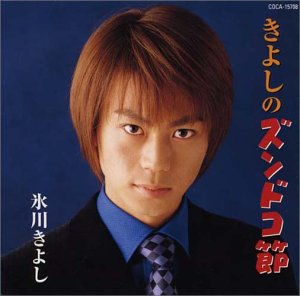
\includegraphics[width=10cm,height=\textheight]{images/kiyoshi.jpg}
    \caption{KIYOSHI\label{kiyoshi}}
    \label{fig:kiyoshi.jpg}
\end{figure}

\section{表}

うひょ〜〜〜〜な表(表\ref{uhyo})

\begin{longtable}[]{@{}rllc@{}}
    \tabularnewline
    \toprule
    卒 & 業 & 論 & 文
    \tabularnewline
    \midrule
    \endfirsthead
    右 & 左 & 標準 & 中央
    \tabularnewline
    わん! & にゃーん & yeah & ぴよぴよ
    \tabularnewline
    \bottomrule
    
    \caption{うひょ〜〜〜〜\label{uhyo}}
\end{longtable}

\section*{謝辞}
